\section{Appendix}

\subsection{Signals Time Domain Statistical Analysis}
\begin{figure}[H]
 % First
\begin{subfigure}{.5\textwidth}
  \centering
  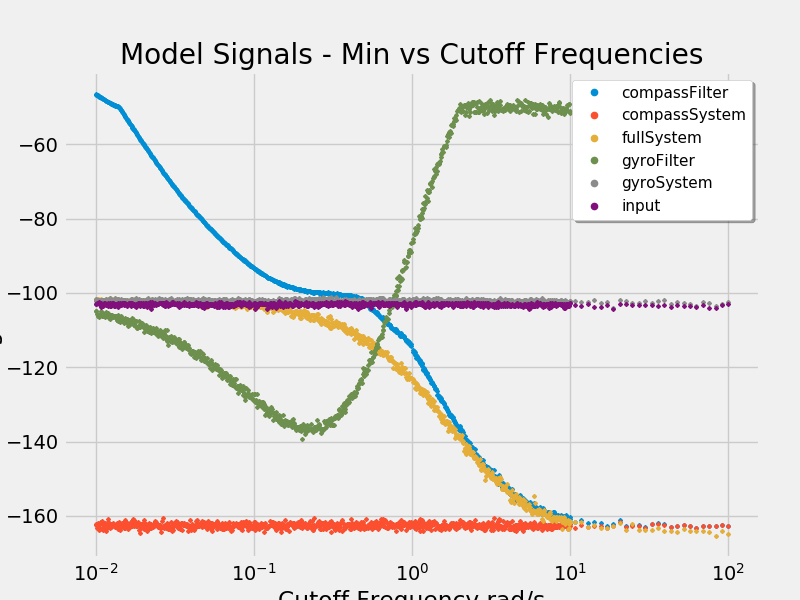
\includegraphics[width=\linewidth, height=\paperheight/5]{img/iterable/modelSignals/modelminSignals.png}  
  \caption{Signals minimum value.}
  \label{fig:model_min}
\end{subfigure}
% Second
\begin{subfigure}{.5\textwidth}
  \centering
  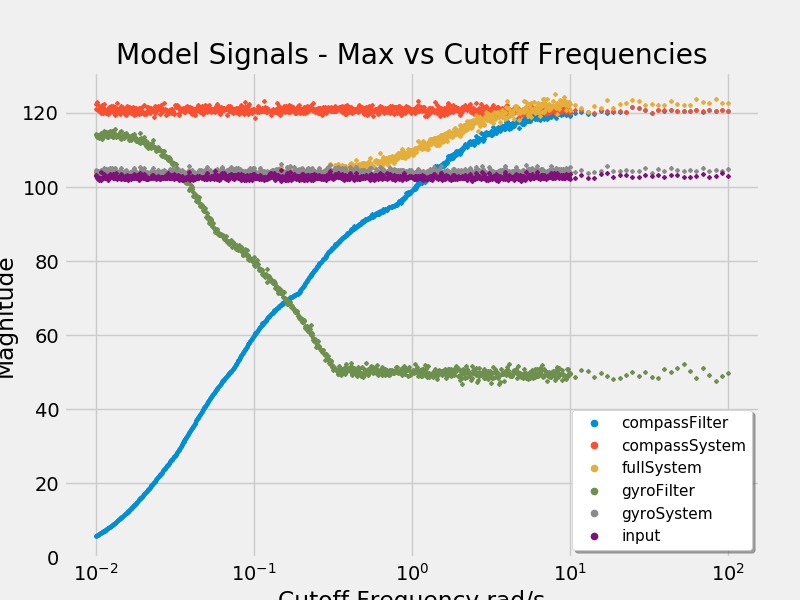
\includegraphics[width=\linewidth, height=\paperheight/5]{img/iterable/modelSignals/modelmaxSignals.png} 
  \caption{Signals maximum value.}
  \label{fig:model_max}
\end{subfigure}
% Third
\begin{subfigure}{.5\textwidth}
\centering
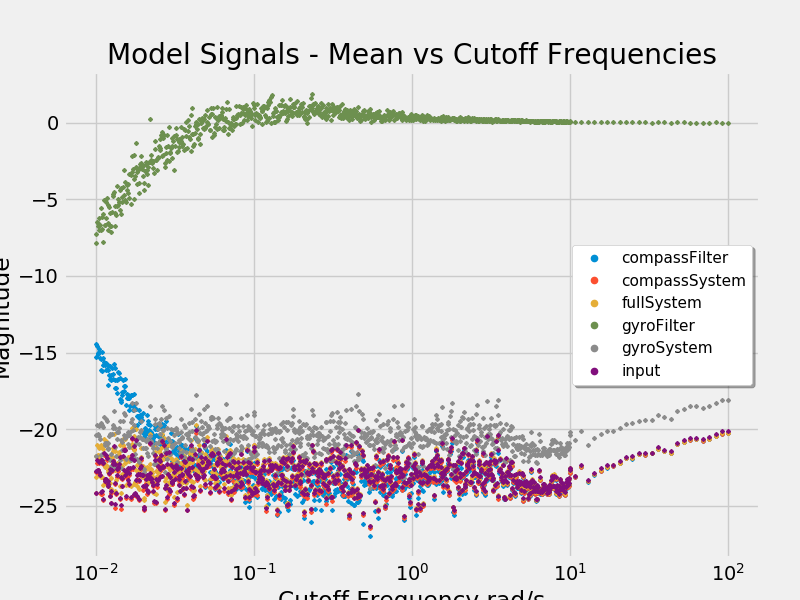
\includegraphics[width=\linewidth, height=\paperheight/5]{img/iterable/modelSignals/modelmeanSignals.png}  
  \caption{Signals mean value ($\propto1^{st}$ Moment)}
\label{fig:model_mean}
\end{subfigure}
  % Fourth
\begin{subfigure}{.5\textwidth}
  \centering
  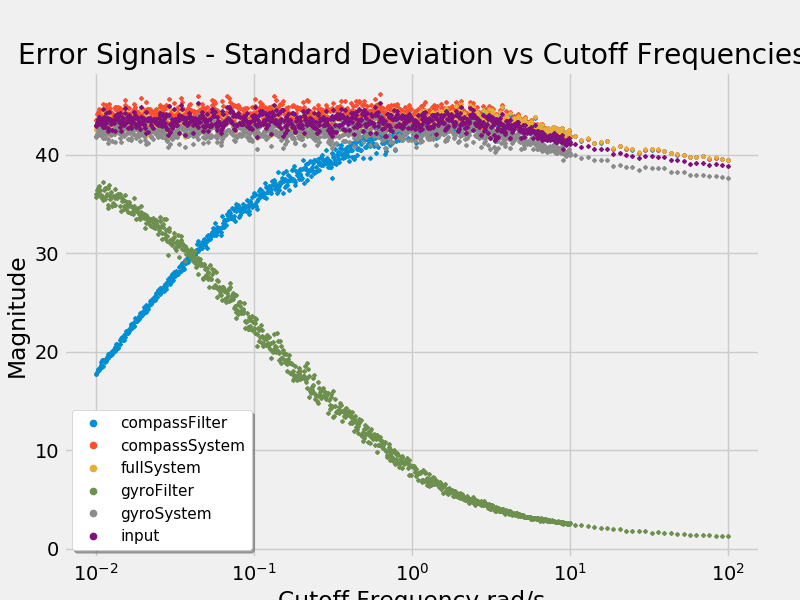
\includegraphics[width=\linewidth, height=\paperheight/5]{img/iterable/modelSignals/modelstandardDeviationSignals.png}  
  \caption{Signals standard deviation. ($\propto2^{nd}$ Moment)}
  \label{fig:model_standard_deviation}
\end{subfigure}
% Fifth
\begin{subfigure}{.5\textwidth}
  \centering
  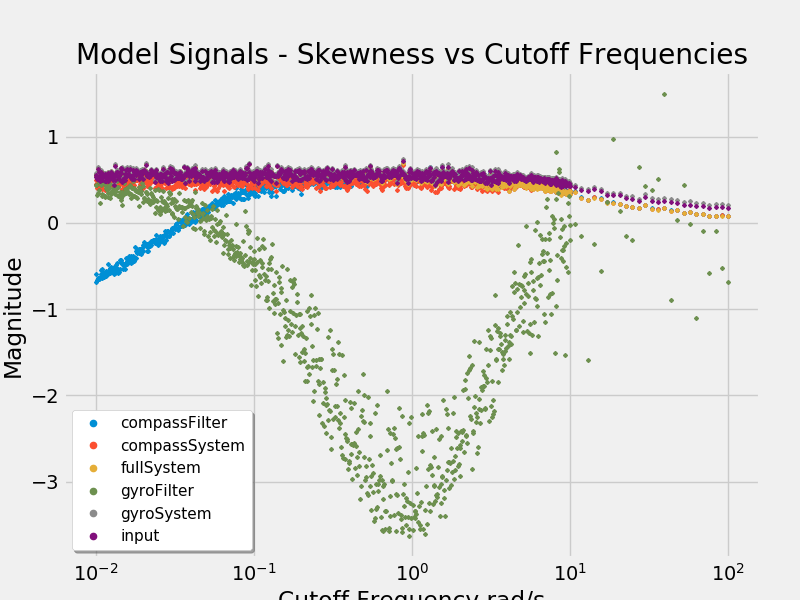
\includegraphics[width=\linewidth, height=\paperheight/5]{img/iterable/modelSignals/modelskewnessSignals.png}  
  \caption{Signals skewness. ($\propto3^{rd}$ Moment)}
  \label{fig:model_skewness}
\end{subfigure}
  % Sixth
\begin{subfigure}{.5\textwidth}
  \centering
  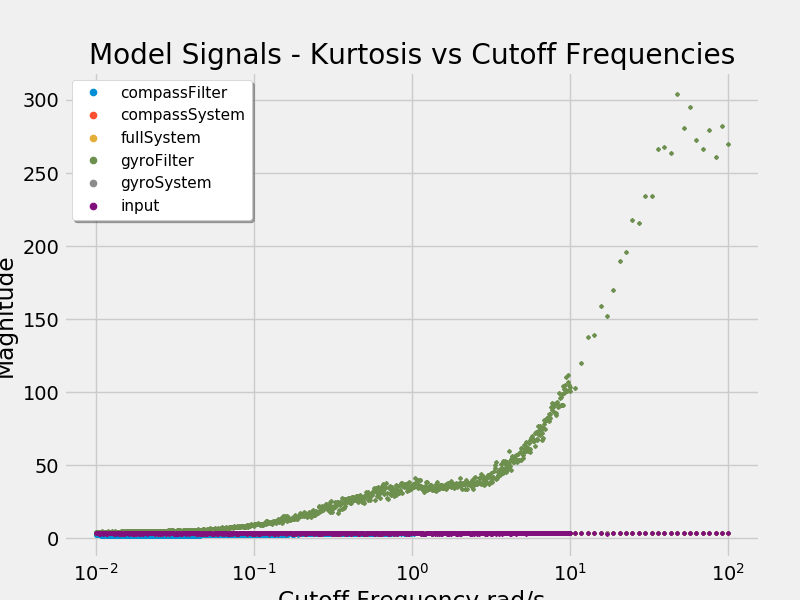
\includegraphics[width=\linewidth, height=\paperheight/5]{img/iterable/modelSignals/modelkurtosisSignals.png}  
  \caption{Signals kurtosis ($\propto4^{th}$ Moment)}
  \label{fig:model_kurtosis}
\end{subfigure}
% Seventh
\begin{subfigure}{.5\textwidth}
  \centering
  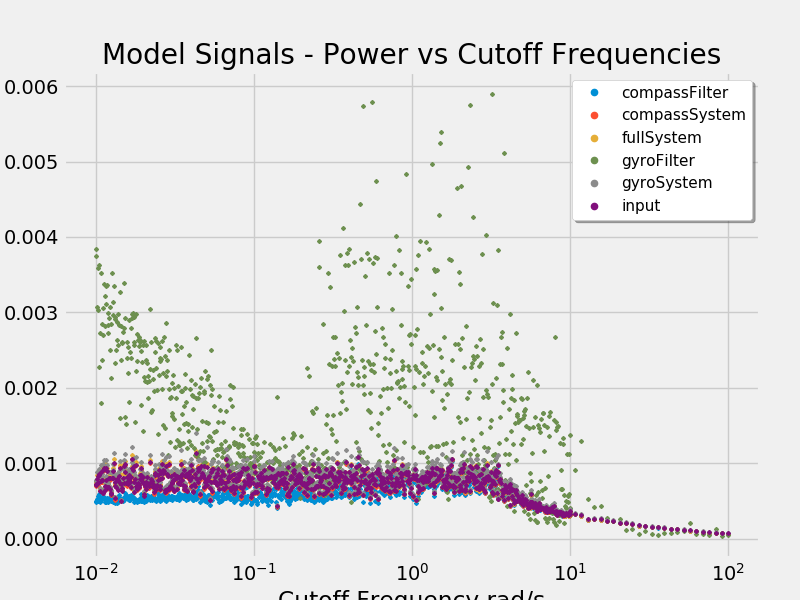
\includegraphics[width=\linewidth, height=\paperheight/5]{img/iterable/modelSignals/modelpowerSignals.png}  
  \caption{Signals 3dB power bandwidth}
  \label{fig:model_power}
\end{subfigure}
\begin{subfigure}{.5\textwidth}
  \centering
  % Eigth
  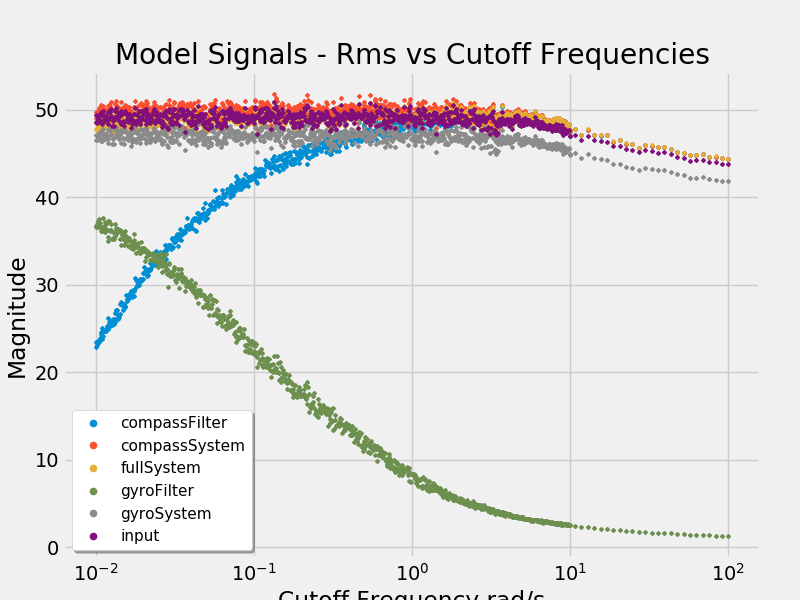
\includegraphics[width=\linewidth, height=\paperheight/5]{img/iterable/modelSignals/modelrmsSignals.png}  
  \caption{Signals RMS (Energy)}
  \label{fig:model_rms}
\end{subfigure}
\caption{Signals time-domain statistical analysis.}
\label{fig:sample_statistical_metrics}
\end{figure}

\subsection{Cutoff Frequency Variation Code}
\label{sec:cutoff_error_variation_code}
\inputminted{octave}{code/errorCutoffFrequencyVariation.m}

\subsection{Heading Signal MATLAB System Block}
\label{sec:heading_signal_code}
\inputminted{octave}{code/HeadingSignals.m}

